\documentclass[a4paper,11pt]{article}
\usepackage{amsmath,amsthm,amsfonts,amssymb,amscd,amstext,vmargin,graphics,graphicx,tabularx,multicol} \usepackage[french]{babel}
\usepackage[utf8]{inputenc}  
\usepackage[T1]{fontenc} 
\usepackage[T1]{fontenc}
\usepackage{amsmath,amssymb}
\usepackage{pstricks-add,tikz,tkz-tab,variations}
\usepackage[autolanguage,np]{numprint} 

\setmarginsrb{1.5cm}{0.5cm}{1cm}{0.5cm}{0cm}{0cm}{0cm}{0cm} %Gauche, haut, droite, haut
\newcounter{numexo}
\newcommand{\exo}[1]{\stepcounter{numexo}\noindent{\bf Exercice~\thenumexo} : \marginpar{\hfill /#1}}
\reversemarginpar
\newcommand{\initexo}{\setcounter{numexo}{0}}



\newcounter{enumtabi}
\newcounter{enumtaba}
\newcommand{\q}{\stepcounter{enumtabi} \theenumtabi.  }
\newcommand{\qa}{\stepcounter{enumtaba} (\alph{enumtaba}) }
\newcommand{\initq}{\setcounter{enumtabi}{0}}
\newcommand{\initqa}{\setcounter{enumtaba}{0}}

\newcommand{\be}{\begin{enumerate}}
\newcommand{\ee}{\end{enumerate}}
\newcommand{\bi}{\begin{itemize}}
\newcommand{\ei}{\end{itemize}}
\newcommand{\bp}{\begin{pspicture*}}
\newcommand{\ep}{\end{pspicture*}}
\newcommand{\bt}{\begin{tabular}}
\newcommand{\et}{\end{tabular}}
\renewcommand{\tabularxcolumn}[1]{>{\centering}m{#1}} %(colonne m{} centrée, au lieu de p par défault) 
\newcommand{\tnl}{\tabularnewline}

\newcommand{\trait}{\noindent \rule{\linewidth}{0.2mm}}
\newcommand{\hs}[1]{\hspace{#1}}
\newcommand{\vs}[1]{\vspace{#1}}

\newcommand{\N}{\mathbb{N}}
\newcommand{\Z}{\mathbb{Z}}
\newcommand{\R}{\mathbb{R}}
\newcommand{\C}{\mathbb{C}}
\newcommand{\Dcal}{\mathcal{D}}
\newcommand{\Ccal}{\mathcal{C}}
\newcommand{\mc}{\mathcal}

\newcommand{\vect}[1]{\overrightarrow{#1}}
\newcommand{\ds}{\displaystyle}
\newcommand{\eq}{\quad \Leftrightarrow \quad}
\newcommand{\vecti}{\vec{\imath}}
\newcommand{\vectj}{\vec{\jmath}}
\newcommand{\Oij}{(O;\vec{\imath}, \vec{\jmath})}
\newcommand{\OIJ}{(O;I,J)}

\newcommand{\bmul}[1]{\begin{multicols}{#1}}
\newcommand{\emul}{\end{multicols}}


\newcommand{\reponse}[1][1]{%
\multido{}{#1}{\makebox[\linewidth]{\rule[0pt]{0pt}{20pt}\dotfill}
}}

\newcommand{\titre}[5] 
% #1: titre #2: haut gauche #3: bas gauche #4: haut droite #5: bas droite
{
\noindent #2 \hfill #4 \\
#3 \hfill #5

\vspace{-1.6cm}

\begin{center}\rule{6cm}{0.5mm}\end{center}
\vspace{0.2cm}
\begin{center}{\large{\textbf{#1}}}\end{center}
\begin{center}\rule{6cm}{0.5mm}\end{center}
}



\begin{document}
\pagestyle{empty}
\titre{Résolution de problèmes avec les équations}{3ème}{}{}{}

\vspace*{0.5cm}


\exo\\

Trouve un nombre sachant que son triple augmenté de 2 est égal à son double augmenté de 3.\\

\vspace*{0.5cm}


\exo \\

Deux frères, Marc et Jean, possèdent chacun un jardin. L'aire du jardin de Marc vaut les $\dfrac{3}{4}$ de l'aire du jardin de Jean. Les deux frères possèdent en tout 1 470 $ m^{2} $.\\

Quelles sont les aires des jardins de Marc et de Jean  ?\\


\vspace*{0.5cm}

\exo\\

Noah veut acheter des livres qui coûtent le même prix.\\
S'il en achète 7, il lui manque 1,20 euros. S'il en achète 6, il lui reste 3,50 euros.\\

Quel est le prix d'un livre ?\\



\vspace*{0.5cm}
\exo



\bmul{2}

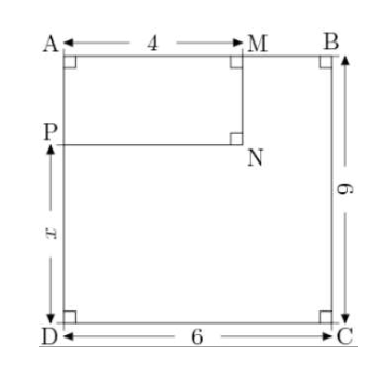
\includegraphics[scale=0.65]{carre.eps} 

\columnbreak

\q Précise,  dans  la  liste ci-dessous,  l'expression  qui  correspond  à l'aire du rectangle AMNP.

\bmul{2}


\qa $4 \times (x-6)$\\

\qa $4 x-6$

\columnbreak

\qa $4 \times (6-x)$\\

\qa $4 \times 6 - x$
\emul




\emul

\q Trouve x pour que l'aire de AMNP soit égale au tiers de l'aire du carré ABCD.\\

\vspace*{0.5cm}


\exo

\bmul{2}
En footing, Anouar et David parcourent la même distance.\\

Anouar part de chez lui, fait trois tours de circuit, puis rentre chez lui.\\
David part de chez lui, fait un tour de circuit, puis rentre chez lui.\\

On note $x$ la longueur, en km, d'un tour de circuit.\\

\columnbreak

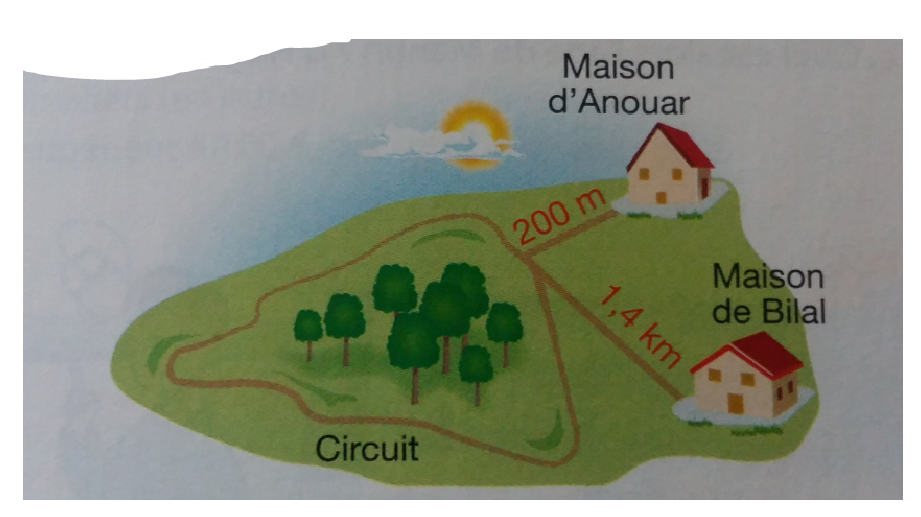
\includegraphics[scale=0.4]{exoapp1.eps} 

\emul

\noindent \initq \q Traduire cette situation par une équation d'inconnue $x$.\\
\q Résoudre cette équation.\\
\q Quelle distance a parcouru chaque ami.\\

\newpage
\vspace*{0.5cm}

\exo

\bmul{2}

$x$ désigne un nombre supérieur à 1.\\
ABCD est un trapèze dont les côtés parallèles [AD] et [BC] ont des longueurs variables.\\

Existe-t-il un nombre $x$ pour lequel ABCD est un parallélogramme ?\\
Si oui, préciser la nature de ABCD dans ce cas.\\

\columnbreak

\begin{center}

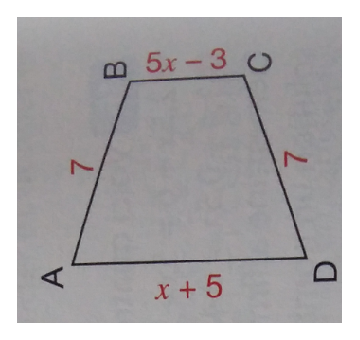
\includegraphics[scale=0.7]{exoapp2.eps} 
\end{center}

\emul

\vspace*{0.5cm}

\exo

\bmul{2}

Le point M se déplace sur le segment [BC]. \\
Est-il possible que les rectangles ABM et DCM aient la même aire ?\\ Justifier votre réponse.\\

\columnbreak

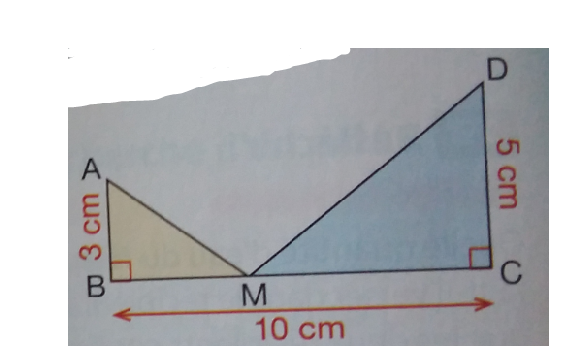
\includegraphics[scale=0.55]{exoapp3.eps} 

\emul

\vspace*{0.5cm}

\exo \\

Résoudre l'équation $(x-1)(x+3)=(x+5)(x-4)$.

\end{document}
